%%%%%%%%%%%%%%%%%%%%%%%%%%%%%%%%%%%%%%%%%%%%%%%%%%%%%%%%%%%%%%%%%%%%%%%
% 1. Document class
%%%%%%%%%%%%%%%%%%%%%%%%%%%%%%%%%%%%%%%%%%%%%%%%%%%%%%%%%%%%%%%%%%%%%%%

\documentclass[a4paper,12pt]{article}

%%%%%%%%%%%%%%%%%%%%%%%%%%%%%%%%%%%%%%%%%%%%%%%%%%%%%%%%%%%%%%%%%%%%%%%
% 2. Packages
%%%%%%%%%%%%%%%%%%%%%%%%%%%%%%%%%%%%%%%%%%%%%%%%%%%%%%%%%%%%%%%%%%%%%%%

% Tipo de input encoding
\usepackage[utf8]{inputenc}
\usepackage[spanish]{babel}

% Margen del documento
\usepackage[top = 2.5cm, bottom = 2.5cm, left = 2.5cm, right = 2.5cm]{geometry} 

% Para crear tablas
\usepackage{multirow}
\usepackage{booktabs}
\usepackage[table,xcdraw]{xcolor}

% Para manejo de gráficos y figuras
\usepackage{graphicx}
\usepackage{natbib}
\usepackage{float}

% Párrafos
\usepackage{setspace}
%\setlength{\parindent}{0cm}
%\setlength{\parskip}{1em}
%\renewcommand{\baselinestretch}{1.5}

% Cambiar el estilo de las listas
\renewcommand{\labelitemi}{$\bullet$}

% Para crear headers
\usepackage{fancyhdr}

% Para bibliografía
\usepackage{natbib}
\set

%%%%%%%%%%%%%%%%%%%%%%%%%%%%%%%%%%%%%%%%%%%%%%%%%%%%%%%%%%%%%%%%%%%%%%%
% 3. Header
%%%%%%%%%%%%%%%%%%%%%%%%%%%%%%%%%%%%%%%%%%%%%%%%%%%%%%%%%%%%%%%%%%%%%%%

% Crear el header
\pagestyle{fancy}
\fancyhf{}
\lhead{\footnotesize Reto I}
\rhead{\footnotesize Grupo 5}

% Colocar el número de la página
\cfoot{\footnotesize \thepage} 

%%%%%%%%%%%%%%%%%%%%%%%%%%%%%%%%%%%%%%%%%%%%%%%%%%%%%%%%%%%%%%%%%%%%%%%
% 4. Title
%%%%%%%%%%%%%%%%%%%%%%%%%%%%%%%%%%%%%%%%%%%%%%%%%%%%%%%%%%%%%%%%%%%%%%%

\begin{document}

\thispagestyle{empty}

% Header de la primera página
\begin{tabular}{p{14cm}}
{\large \bf Análisis Numérico} \\
Pontificia Universidad Javeriana \\ Semestre 2021-10 \\
\hline
% \\
\end{tabular}

% Título
\title{Reto I}
\author{Alejandro Morales Contreras \\ Carlos Miguel Sánchez Loreto \\ Santiago Vásquez Sánchez}
\date{}

\begingroup
\let\newpage\relax
\maketitle
\endgroup

%%%%%%%%%%%%%%%%%%%%%%%%%%%%%%%%%%%%%%%%%%%%%%%%%%%%%%%%%%%%%%%%%%%%%%%
% 5. Body
%%%%%%%%%%%%%%%%%%%%%%%%%%%%%%%%%%%%%%%%%%%%%%%%%%%%%%%%%%%%%%%%%%%%%%%

\section{Introducción}

%\setlength{\parskip}{1em}

El presente documento pretende mostrar el análisis, implementación y resultados obtenidos del reto I de la materia sobre el algoritmo de Brent, intersección entre curvas y librerías para la solución de raíces. La implementación de los algoritmos fue llevada a cabo en el lenguaje de programación R, y los resultados fueron comparados mediante la herramienta Wolfram Alpha.

%%%%%%%%%%%%%%%%%%%%%%%%%%%%%%%%%%%%%%%%%%%%%%%%%%%%%%%%%%%%%%%%%%%%%%%
% 5.1 Algoritmo de Brent
%%%%%%%%%%%%%%%%%%%%%%%%%%%%%%%%%%%%%%%%%%%%%%%%%%%%%%%%%%%%%%%%%%%%%%%

\section{Algoritmo de Brent}

Es un algoritmo iterativo que calcula la raíz de la función $f(x)$ en un intervalo $[a,b]$. El algoritmo de Brent, es en verdad, múltiples implementaciones de algoritmos ya existentes para el cálculo de la raíces de un polinomio. Utiliza los métodos: interpolación inversa cuadrática, el método de la secante, y el método de la bisección. Por cada iteración, el algoritmo evalúa cual es el método adecuado para la aproximación actual, y con este calcula el siguiente paso. \cite{fuente_oconnor_ingenierialgoritmos_2017} \par

Este método suele converger muy rápidamente a cero; para las funciones difíciles
ocasionales que se encuentran en la práctica. \par 

\subsection{Condiciones del Algoritmo}

Para aplicar el método para calcular la raíz de la función $f(x)$ en un intervalo $[a,b]$, se deben cumplir las siguientes condiciones:

\begin{enumerate}
    \item $f(x)$ debe ser continua y derivable en el intervalo $[a,b]$
    \item $f(a) \cdotp f(b) < 0$, es decir, existe una raíz para $f(x)$ en $[a,b]$
\end{enumerate}

\newpage

\subsection{Explicación del Algoritmo}

El algoritmo de Brent es un método iterativo. Esto quiere decir que para hallar el valor de $x$ en la iteración $i+1$, se debe conocer el valor de $x$ en la iteración $i$, y operar desde este. El método trabaja en verdad con tres puntos, $x_0$, $x_1$, $x_2$. \par

Como se mencionó anteriormente, el algoritmo de Brent es híbrido, incorporando el de interpolación cuadrática inversa, el método de la secante y el método de la bisección. El algoritmo consiste en, por cada paso, evaluar el método adecuado dadas unas condiciones, y con este aproximar a la raíz de la función. \par 

A continuación se presentan las fórmulas que modelan cada uno de los métodos que son utilizados por el algoritmo de Brent. Se asume que $a=x_0$, $b=x_1$, $c=x_2$. \par

La fórmula que modela el método de interpolación cuadrática inversa es: \par 

\[ s = \frac{af(b)f(c)}{(f(a)-f(b))(f(a)-f(c))} + \frac{bf(a)f(c)}{(f(b)-f(a))(f(b)-f(c))} + \frac{cf(b)f(c)}{(f(c)-f(a))(f(c)-f(b))} \]

La fórmula que modela el método de la secante es: \par 

\[ s = b - f(b)\frac{b - a}{f(b) - f(a)} \]

La fórmula que modela el método de la bisección es: \par 

\[ s = \frac{a + b}{2} \]

\newpage

\subsection{Diagrama de Flujo del Algoritmo}

A continuación se presenta el diagrama de flujo que modela cómo se debe implementar el algoritmo de Brent: \par 

\vspace{1em}

% Figura: Diagrama de flujo Brent
\begin{figure}[h!]
\centering
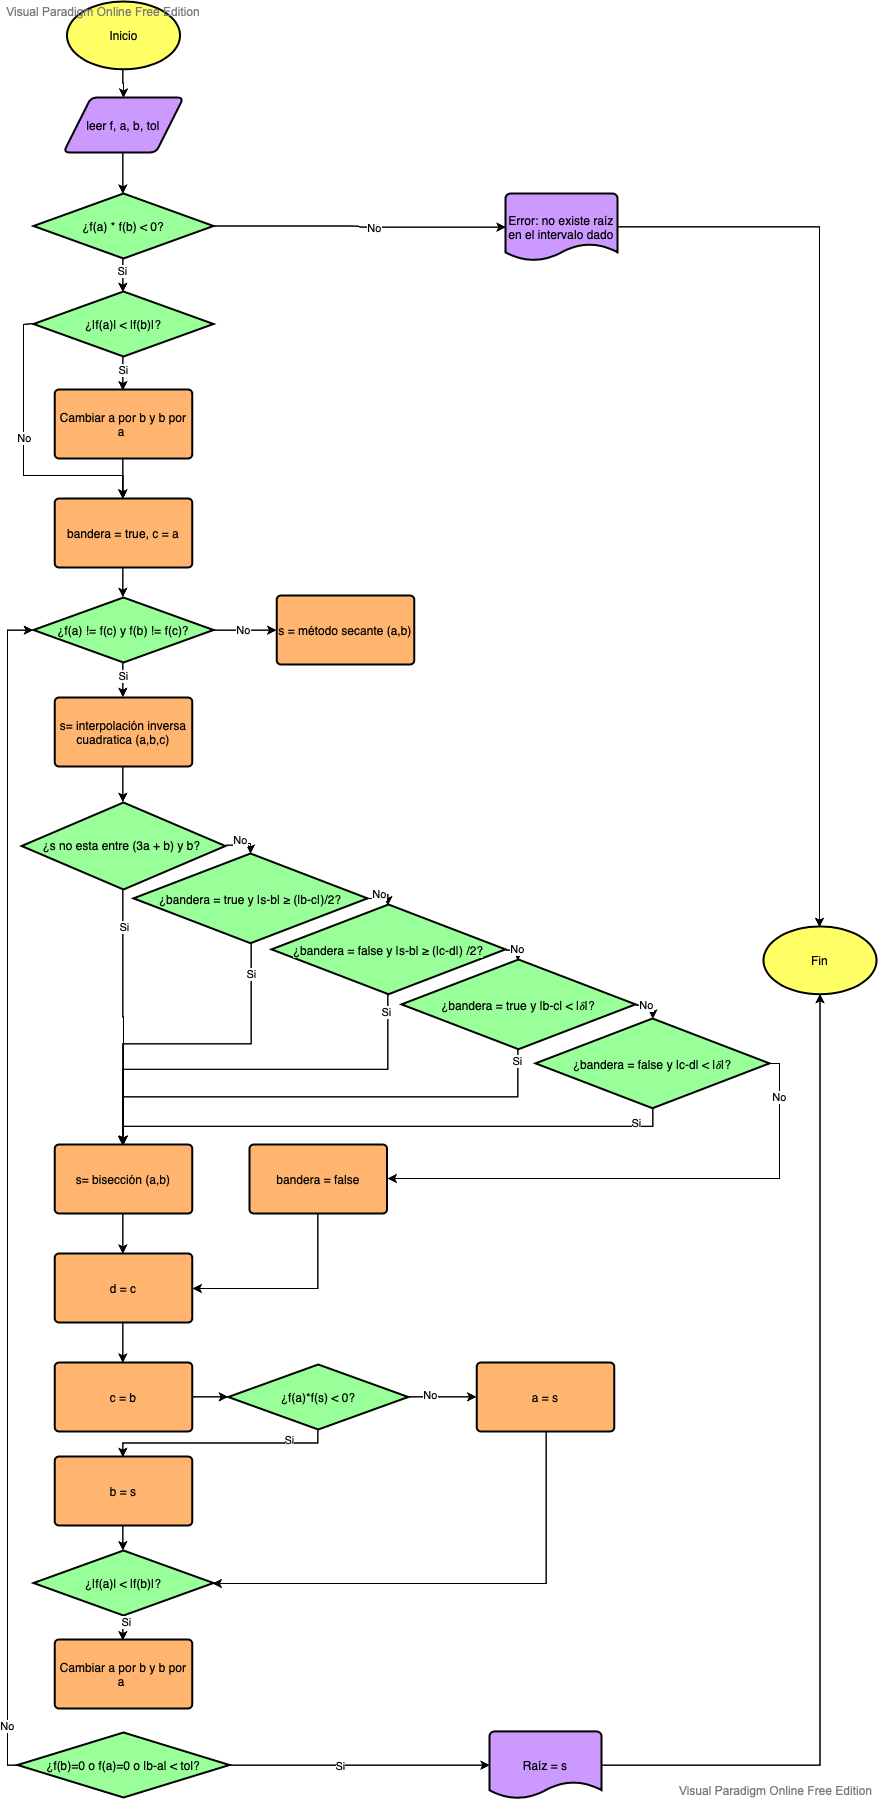
\includegraphics[scale=0.3]{img/flujograma_brent.png}
\vspace{-1em}
\caption{Diagrama de flujo del algoritmo de Brent}
\label{fig:flujograma_brent}
\end{figure}

\newpage

\subsection{Implementación del Algoritmo}

El método fue implementado en R. El código fuente puede ser encontrado en el siguiente repositorio: \par

\vspace{1em}
https://github.com/AlejandroMoralesContreras/analisis-numerico.git \par

\subsubsection{Niveles de Significancia}

Para los niveles de significancia obtenidos aplicando el algoritmo de Brent se utilizaron las tolerancias $10^{-8}$,$10^{-16}$,$10^{-32}$ y $10^{-50}$.
Comparando los resultados con Wolfram Alpha se establece que para una toleracia de $10^{-8}$ el nivel de significancia es alto debido a que de las 8 cifras significativas, 5 de ellas concuerdan con el resultado. A medida que se aumenta la toleracia este nivel de significacia comienza a disminuir considerablemente, hasta obtener una perdida de hasta 43 cifras significativas. \par

\subsubsection{Precisión}

En la implementación del algoritmo de Brent, se utilizó la libreria \textit{Rmpfr} de R con la finalidad de establecer una alta precisión o precisión extendida de 180 bits. Aplicar esta librería le permite al algoritmo trabajar con una mayor cantidad de cifras significativas, y alcanzar una precisión más alta. \par

\subsubsection{Resultados Obtenidos}

El problema consistía en aplicar el algoritmo de Brent para hallar las raíces de la función $f(x)=x^3-2x^2+\frac{4}{3}x-\frac{8}{27}$ con un error menor de $2^{-50}$. \par

A continuación se presentan los resultados obtenidos, la cantidad de iteraciones que le toma al método alcanzar dicho resultado, así como la comparación con el valor real: \par

Se toma como intervalo inicial $a = 0$, $b = 1$ \par

% Volver a generar esta tabla

\begin{table}[ht!]
\begin{tabular}{clc}
Tol      & \multicolumn{1}{c}{x}                                    & i   \\
1.00E-08 & 0.66666987                                               & 137 \\
1.00E-16 & 0.6666698708192892                                       & 139 \\
1.00E-32 & 0.66666987081928920008177594108415                       & 143 \\
1.00E-50 & 0.666669870819289200081775941084153738997637959149       & 160 \\
Wolfram  & 0.666666666666666666666666666666666666666666666666666666 &    
\end{tabular}
\end{table}

\vspace{-1em}
\begin{itemize}
    \item Pérdida de significancia: el algoritmo sufre una gran perdida de significancia debido a que la raíz es periódica.
    \vspace{-10pt}
    \item Número de iteraciones: el algoritmo demora una cantidad de iteraciones relativamente alta, pero si se compara con métodos implementados anteriormente para este tipo particular de funciones, se concluye que en realidad es capaz de calcular la raíz es muy pocas iteraciones.
    \vspace{-10pt}
    \item Convergencia: el algoritmo converge linealmente.
\end{itemize}

\newpage

\subsection{Evaluación de Librerías}

Para obtener la raíz o raíces de un polinomio, R cuenta con distintas funciones y librerías dispuestas para este proceso. A continuación se presentan los resultados obtenidos de evaluar la función $f(x)=x^3-2x^2+\frac{4}{3}x-\frac{8}{27}$. \par 

Las funciones fueron implementadas en R. El código fuente puede ser encontrado en el siguiente repositorio: \par

\vspace{1em}
https://github.com/AlejandroMoralesContreras/analisis-numerico.git \par

\subsubsection{Función polyroot}

La función polyroot es utilizada de la siguiente forma: \par

\begin{verbatim}
polyroot(c(-8/27, 4/3, -2, 1))
\end{verbatim}

A continuación se presentan los resultados obtenidos. \par

\begin{table}[ht!]
\begin{tabular}{cr}
Raíz & \multicolumn{1}{c}{Valor}  \\
$x_0$ & 0.66666666666667018       \\
$x_1$ & 0.66666666666666274       \\
$x_2$ & 0.66666666666666718      
\end{tabular}
\end{table}

Como se puede evidenciar, la función reconoce correctamente la multiplicidad de la raíz, arrojando tres raíces como resultado. Así mismo, los resultados son bastante precisos, alcanzando 14 dígitos de exactitud. Esta función trabaja con precisión doble equivalente hasta el épsilon de la máquina. \par

\subsubsection{Función uniroot}

La función uniroot es utilizada de la siguiente forma: \par

\begin{verbatim}
fx = expression(x^3 - 2*x^2 + (4/3)*x - (8/27))
Fx <- function(x) {{ eval(fx[[1]]) }}
uniroot(Fx, c(0, 1), tol = 10^-16, maxiter=100)
\end{verbatim}

A continuación se presentan los resultados obtenidos. \par

\begin{table}[ht!]
\begin{tabular}{cr}
Salida     & \multicolumn{1}{c}{Valor}                  \\
root       & 0.66666945782102738                        \\
f.root     & 0                                          \\
iter       & 35                                         \\
estim.prec & \multicolumn{1}{l}{1.6779406376343786e-05}
\end{tabular}
\end{table}

Analizando los resultados, se puede evidenciar que la función tiene una pérdida de precisión significativa (verificando tanto el valor root como estim.prec), en 35 iteraciones. Esta función trabaja con precisión doble equivalente hasta el épsilon de la máquina (no puede llegar a tolerancias más altas). \par

\newpage

\subsubsection{Función pracma::brentDekker}

La función brentDekker, de la librería pracma, es utilizada de la siguiente forma: \par

\begin{verbatim}
fx = expression(x^3 - 2*x^2 + (4/3)*x - (8/27))
Fx <- function(x) {{ mpfr(eval(fx[[1]]), 180) }}
brentDekker(Fx, 0, 1, maxiter = 100, tol = mpfr(10^-50, 180))
\end{verbatim}

A continuación se presentan los resultados obtenidos. \par

\begin{table}[ht!]
\begin{tabular}{cr}
Salida     & \multicolumn{1}{c}{Valor}                                \\
root       & 0.6666698708192892000817759410841537389976379276428      \\
f.root     & -6.5253044679985245267102941092565475557011642580689e-55 \\
f.calls    & 64                                                       \\
estim.prec & 3.6685482316111882191172023770915239711091192626887e-39 
\end{tabular}
\end{table}

Analizando los resultados, se puede evidenciar que la función tiene una pérdida de precisión significativa (verificando tanto el valor root como estim.prec), en 64 iteraciones. Esta función se pudo adaptar mediante el uso de la librería Rmpfr, trabajando con precisión extendida de 180 bits. \par

\subsubsection{Función rootSolve::uniroot.all}

La función uniroot.all, de la librería rootSolve, es utilizada de la siguiente forma: \par

\begin{verbatim}
fx = expression(x^3 - 2*x^2 + (4/3)*x - (8/27))
Fx <- function(x) {{ eval(fx[[1]]) }}
uniroot.all(Fx, c(0, 1), tol = 10^-16, maxiter=100)
\end{verbatim}

A continuación se presentan los resultados obtenidos. \par

\vspace{1em}
$x=0.66666970767641276$
\vspace{1em}

Analizando los resultados, se puede evidenciar que la función tiene una pérdida de precisión significativa (verificando tanto el valor root como estim.prec), después del quinto digito decimal. Esta función trabaja con precisión doble equivalente hasta el épsilon de la máquina (no puede llegar a tolerancias más altas). \par

\newpage

\subsection{Pruebas}

\subsubsection{Raíces múltiples}

Para evaluar la multiplicidad de las raíces, se utiliza la definición de las derivadas de la función.

\[ f(x)=x^3 -2x^2 + \frac{4x}{3} -\frac{8}{27} \textrm{ donde } f(x)=0 \textrm{ es } x = \frac{2}{3} \]

\[ f'(x)=\frac{1}{3}(2-3x)^2 \textrm{ donde } f'(x)=0 \textrm{ es } x = \frac{2}{3} \]

\[ f''(x)=6x-4 \textrm{ donde } f'(x)=0 \textrm{ es } x = \frac{2}{3} \]

De este modo se determina entonces que la función $f(x)$ tiene raiz de multiplicidad 3. \par

\subsubsection{Capacidad de la máquina}

Se encontró que el épsilon de la máquina ($\epsilon_{maq} \approx 2.22 \times 10^{-16}$) impedía alcanzar la tolerancia deseada, de $10^{-50}$. Por ende, se hizo uso de la librería \emph{Rmpfr} para aumentar la precisión de las operaciones. \par 

\newpage 

\subsection{Orden de Convergencia}

El orden de convergencia del método se verifica mediante la fórmula: \par

\[ 0 \leq \lim_{i\to\infty} \frac{|x_{i+1}-x^*|}{|x_i-x^*|^r} < \infty \]

donde $r$ es el máximo entero positivo que satisface la fórmula, y representa el orden de convergencia. Al hacer los cálculos para la función evaluada, se encuentra que $r=1$. Esto confirma que el algoritmo converge linealmente. \par

Este resultado de convergencia lineal no es extraño. Aunque el algoritmo de Brent es óptimo frente a problemas en los que otros métodos fallan, el problema planteado tiene una raíz muy particular. Esta raíz tiene multiplicidad de 3 (Se ha demostrado entregas que una mayor multiplicidad de la raíz representa más dificultad para encontrarla). Así mismo, es una raíz de fracción periódica. \par

\subsection{Eficiencia del Algoritmo} 

Se mide la eficiencia del algoritmo mediante el tiempo de ejecución, la pérdida de signifcancia y la cantidad de iteraciones que le toma alcanzar la tolerancia. Se evaluó la función $f(x)=x^3-2x^2+\frac{4}{3}x-\frac{8}{27}$ en el intervalo $[0,1]$ con una tolerancia de $10^{-50}$. \par 

\subsubsection{Tiempo de ejecución}

El tiempo de ejecución se midió mediante el uso de las funciones del sistema, disponibles en R. Se realizaron tres pruebas y se calculó el promedio de estas para determinar el tiempo de ejecución del algoritmo.  En la siguiente tabla se registran los resultados obtenidos: \par 

\begin{table}[ht!]
\begin{tabular}{cc}
Prueba & Tiempo de ejecución (segundos) \\
1      & 5.094451                       \\
2      & 5.090444                       \\
3      & 5.076924                       \\
Prom   & 5.087273                      
\end{tabular}
\end{table}
\vspace{-1em}

\subsubsection{Pérdida de Significancia}

El algoritmo de Brent es inusualmente bueno para resolver problemas en el que otros algoritmos divergen, en este caso especifico el algoritmo tiene una perdida de significancia alta puesto que  la raíz tiene multiplicidad de 3 y es una fracción periódica. Estas caracteristicas hacen que el algoritmo tenga una mayor dificultad para encontrar la raiz y por lo tento tenga una perdida de significancia mayor.\par 

\subsubsection{Cantidad de Iteraciones}

Este algoritmo generalmente calcula las raíces de una función en una cantidad de iteraciones muy baja, convergiendo rapidamente a cero, pero cuando se trabajan tipos de funciones particulares con raíces periódicas o imaginarias, utiliza un número más grande de iteraciones, sin embargo, en comparación con otros métodos como Newton-Raphson Relajado o el método de Bisección este algoritmo posee una convergencia mucho más acelerada y por lo tanto es capaz de calcular las raíces de una función en relativamente pocas iteraciones. \par 

\newpage 

\subsection{Comparaciones}

Con el fin de analizar más profundamente el algoritmo de Brent, se realiza una comparación contra otros métodos. A continuación se presentan los resultados obtenidos de evaluar la función $f(x)=x^3-2x^2+\frac{4}{3}x-\frac{8}{27}$. \par

\subsubsection{Comparación contra el Método Newton-Rhapson Relajado}

A continuación se presentan los resultados comparativos entre el método Newton-Rhapson Relajado y el algoritmo de Brent. Se evalúan ambos con una tol de $10^{-50}$. \par

\begin{table}[ht!]
\begin{tabular}{crr}
        & \multicolumn{1}{c}{x}                                & \multicolumn{1}{c}{i} \\
NRR     & 0.67311616206344526691651708460994996130466461181640 & 4000                  \\
Brent   & 0.66666987081928920008177594108415373899763795914909 & 161                   \\
Wolfram & 0.66666666666666666666666666666666666666666666666667 & \multicolumn{1}{l}{} 
\end{tabular}
\end{table}

Analizando los resultados, se puede determinar que el algoritmo de Brent es más preciso y eficiente que el método Newton-Rhapson Relajado. Así mismo, le toma menos iteraciones alcanzar una precisión más alta. \par

\subsubsection{Comparación contra el Método de la Bisección}

A continuación se presentan los resultados comparativos entre el método de la bisección y el algoritmo de Brent. Se evalúan ambos con una tol de $10^{-50}$. \par

\begin{table}[ht!]
\begin{tabular}{crr}
          & \multicolumn{1}{c}{x}                                & \multicolumn{1}{c}{i} \\
Bisección & 0.66666987081928920008177594108415373899763792973914 & 143                   \\
Brent     & 0.66666987081928920008177594108415373899763795914909 & 161                   \\
Wolfram   & 0.66666666666666666666666666666666666666666666666667 & \multicolumn{1}{l}{} 
\end{tabular}
\end{table}

Analizando los resultados, se puede determinar ambos métodos tienen un comportamiento muy similar. Este resultado no es de extrañar, debido a que el algoritmo de Brent implementa al método de la bisección para aquellos casos en los que se cumplan las condiciones. Para la función evaluada, el método de la bisección termina siendo utilizada bastantes veces por Brent. \par

\newpage

\subsection{Gráficas Comparativas}

\subsubsection{Relación entre Error contra Iteraciones}

A continuación se presenta la gráfica que modela la relación entre la cantidad de iteraciones que le toma al método obtener la raíz y el error calculado para esa iteración. El análisis se realizó a partir de la función $f(x)=x^3-2x^2+\frac{4}{3}x-\frac{8}{27}$ con intervalo inicial $[0,1]$. \par

% Figura: Error contra Iteraciones brent
\vspace{-2em}
\begin{figure}[ht!]
\centering
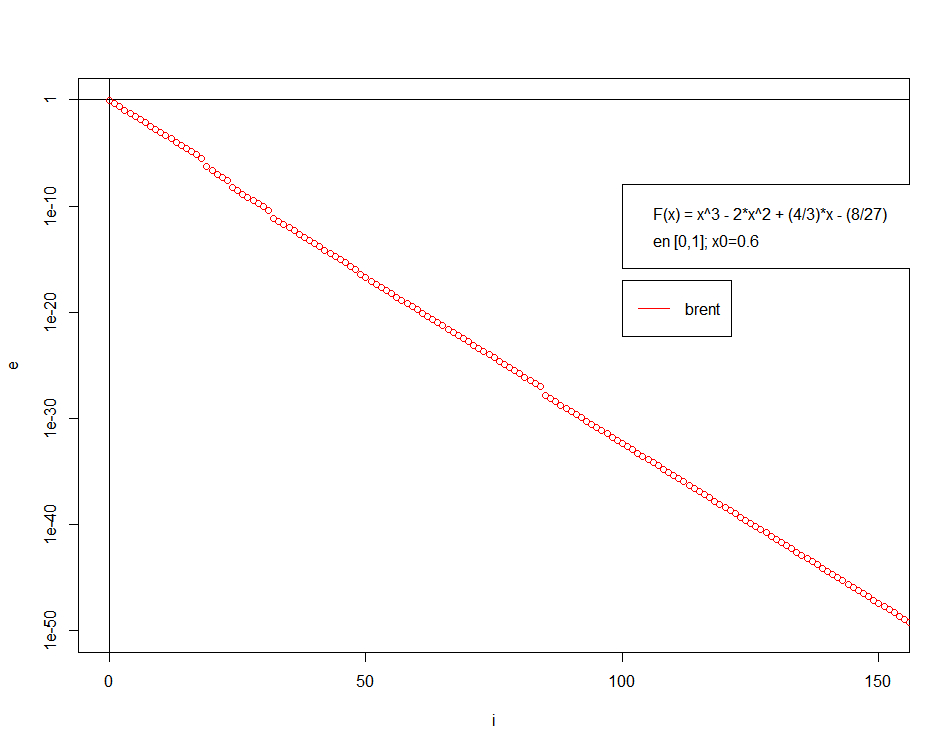
\includegraphics[scale=0.4]{img/brent_e_vs_i.png}
\vspace{-1em}
\caption{Error vs. Iteraciones del algoritmo de Brent}
\label{fig:brent_e_i}
\end{figure}

\vspace{-1em}

\subsubsection{Relación entre $\varepsilon_i$ y $\varepsilon_{i+1}$}

A continuación se presenta la gráfica que relaciona $\varepsilon_i$ con $\varepsilon_{i+1}$ para el algoritmo de Brent. \par

% Figura: Relación entre Ei y Ei+1 brent
\vspace{-1em}
\begin{figure}[ht!]
\centering
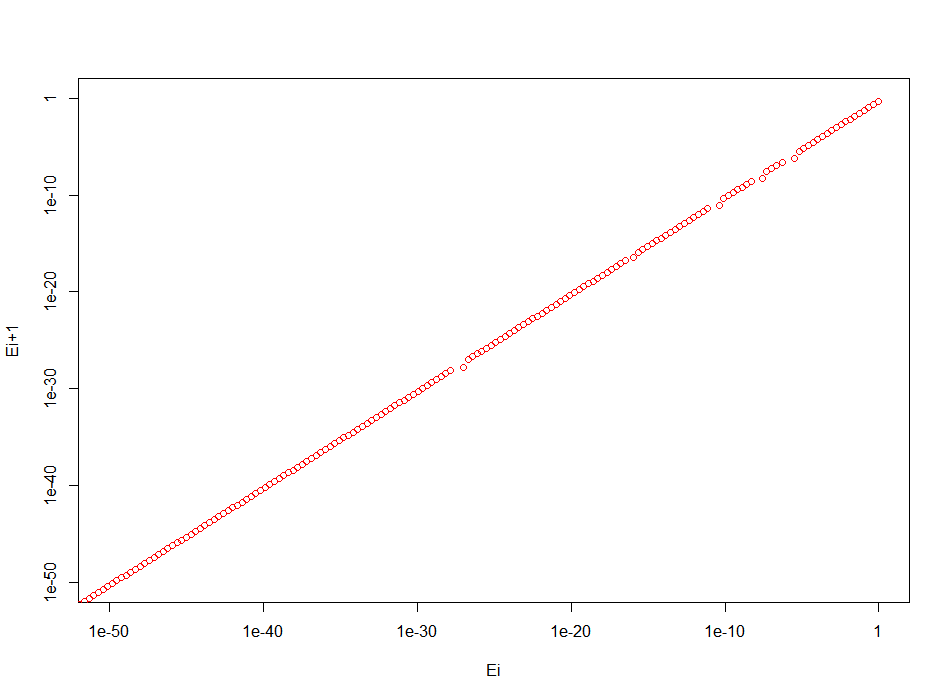
\includegraphics[scale=0.4]{img/brent_relacion_error.png}
\vspace{-1em}
\caption{Relación entre $\varepsilon_i$ y $\varepsilon_{i+1}$ del algoritmo de Brent}
\label{fig:relacion_error_brent}
\end{figure}

\newpage

\subsubsection{Comparación contra otros métodos}

A continuación se presenta la gráfica que compara la convergencia del algoritmo de Brent, con las del método Newton-Raphson Relajado y el método de la bisección. El análisis se realizó a partir de la función $f(x)=x^3-2x^2+\frac{4}{3}x-\frac{8}{27}$ en el intervalo $[0,1]$ con punto inicial $x_0 = 1$. \par

% Figura: Brent vs metodos
\vspace{-1em}
\begin{figure}[ht!]
\centering
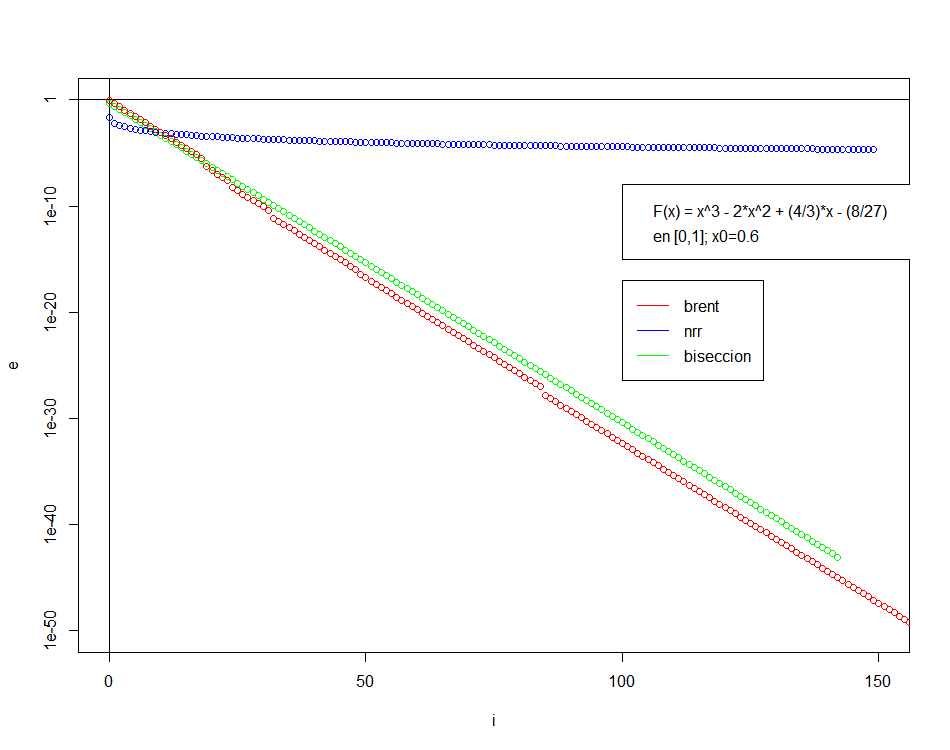
\includegraphics[scale=0.6]{img/brent_vs_metodos.png}
\vspace{-1em}
\caption{Comparación del algoritmo de Brent contra otros métodos}
\label{fig:brent_vs_metodos}
\end{figure}

\newpage

%%%%%%%%%%%%%%%%%%%%%%%%%%%%%%%%%%%%%%%%%%%%%%%%%%%%%%%%%%%%%%%%%%%%%%%
% 5.2 Intersección de Raíces
%%%%%%%%%%%%%%%%%%%%%%%%%%%%%%%%%%%%%%%%%%%%%%%%%%%%%%%%%%%%%%%%%%%%%%%

\section{Intersección entre curvas}

Para poder determinar la intersección entre curvas, se pueden aplicar los métodos para calcular las raíces de un polinomio. Esto se debe a que la intersección entre dos curvas se puede representar como la resta de las ecuaciones que las modelan. Esta resta resulta en una nueva función. Si esta se iguala a 0, es posible determinar la raíz de la función. Esta raíz va a ser la intersección entre las curvas evaluadas. \par 

A continuación se va a presentar este proceso para calcular la intersección entre dos curvas, y después se procederá a resolver mediante el método de Newton-Rhapson relajado. \par 

\subsection{Condiciones del Algoritmo}

Para aplicar el método para calcular la intersección de dos curvas $f(x)$ y $g(x)$ en un intervalo $[a,b]$, se deben cumplir las siguientes condiciones:

\begin{enumerate}
    \item $f(x)$ debe ser continua y derivable en el intervalo $[a,b]$
    \item $g(x)$ debe ser continua y derivable en el intervalo $[a,b]$
    \item Se deben poder expresar las funciones como $h(x)=f(x)-g(x)$
    \item $h(a) \cdotp h(b) < 0$, es decir, existe una raíz para $h(x)$ en $[a,b]$
\end{enumerate}

\subsection{Explicación del Algoritmo}

Para calcular la intersección entre dos curvas modeladas por dos ecuaciones $ec_1$ y $ec_2$, se puede aplicar el truco de restar ambas y encontrar la encontrar la raíz de la función generada. Este truco funciona, debido a que la resta de ambas dos ecuaciones es equivalente a su igualación. La igualación es uno de los métodos algebráicos básicos para resolver un sistema de ecuaciones. \par

Dadas dos ecuaciones  $ec_1$ y $ec_2$, el proceso de hallar su intersección consiste entonces en: \par

\begin{enumerate}
    \item Expresar $ec_1$ como $y=f(x)$ y $ec_2$ como $y=g(x)$. Esto se logra despejando las ecuaciones por el término y
    \item Calcular $h(x)=f(x)-g(x)$
	\item Hallar la raíz de la nueva función $x_0=h(x)$ mediante un método para calcular las raíces de un polinomio
	\item Calcular $y_0=f(x_0)$
\end{enumerate}

Al final, $(x_0, y_0)$ será el punto que representa la intersección entre las dos curvas. \par 

Para propósitos de este reto, el método escogido para calcular la raíz de la función $h(x)$ generada es el método Newton-Rhapson Relajado. \par 

\newpage

\subsection{Diagrama de Flujo del Algoritmo}

\subsubsection{Intersección entre curvas}

A continuación se presenta el diagrama de flujo que modela cómo se debe implementar el proceso para calcular la intersección entre dos curvas. \par 

\vspace{1em}

% Figura: Diagrama de flujo interseccion de curvas
\begin{figure}[h!]
\centering
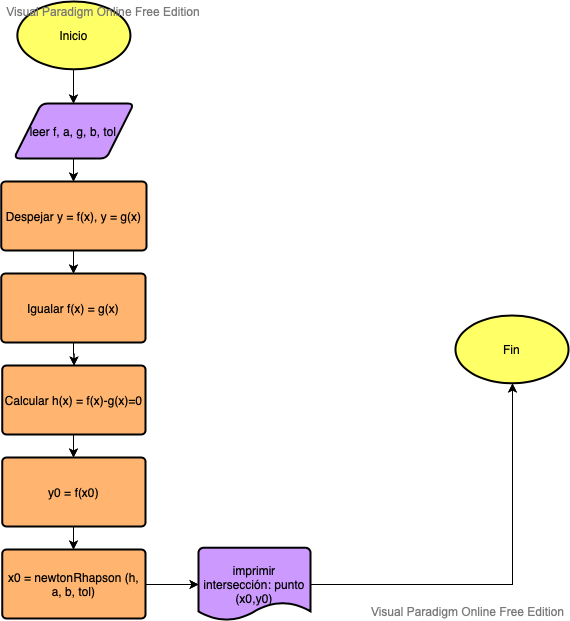
\includegraphics[scale=0.7]{img/flujograma_interseccion.png}
\vspace{-1em}
\caption{Diagrama de flujo de la intersección de curvas}
\label{fig:flujograma_interseccion}
\end{figure}

\newpage

\subsubsection{Método Newton-Rhapson Relajado}

El diagrama de flujo que representa cómo se debe implementar el método Newton-Rhapson Relajado se presenta a continuación.

% Figura: Diagrama de flujo interseccion nrr
\begin{figure}[h!]
\centering
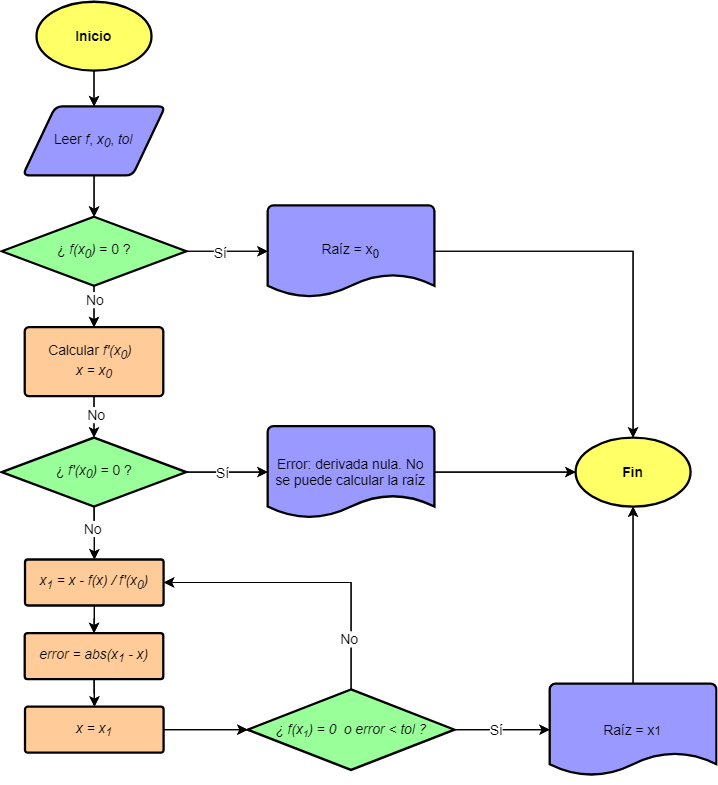
\includegraphics[scale=0.8]{img/flujograma_nrr.png}
\vspace{-1em}
\caption{Diagrama de flujo del método Newton-Rhapson Relajado}
\label{fig:flujograma_nrr}
\end{figure}

\newpage

\subsection{Implementación del Algoritmo}

El método fue implementado en R. El código fuente puede ser encontrado en el siguiente repositorio: \par

\vspace{1em}
https://github.com/AlejandroMoralesContreras/analisis-numerico.git \par

\subsubsection{Niveles de Significancia}

Para los niveles de significancia obtenidos aplicando el algoritmo de Newton-Rhapson Relajado se utilizaron las tolerancias $10^{-8}$,$10^{-16}$,$10^{-32}$ y $10^{-50}$. Los resultados se comparan con Wolfram Alpha, con el fin de verificar la pérdida de significancia en la que pueda incurrir el algoritmo a la hora de calcular la raíz para cada tolerancia dada. \par

\subsubsection{Precisión}

En la implementación del algoritmo de Newthon-Rhapson Relajado, se utilizó la libreria \textit{Rmpfr} de R con la finalidad de establecer una alta precisión o precisión extendida de 180 bits. Aplicar esta librería le permite al algoritmo trabajar con una mayor cantidad de cifras significativas, y alcanzar una precisión más alta. \par

\subsubsection{Resultados Obtenidos}

El problema consistía en calcular la intersección entre las siguientes curvas con un error menor de $10^{-16}$:
\[ x^2 + xy = 10 \textrm{ ; } y + 3xy^2 = 57 \]

Inicialmente, se despejaron ambas ecuaciones en términos de $y$ con ayuda de Wolfram Alpha. Se obtuvieron las siguientes funciones: \par

\[ f(x)=\frac{10}{x}-x \textrm{ ; } g(x)=-\frac{1 \pm \sqrt{1 + 684 x}}{6x} \]

Como se puede ver, para el caso de la función $g(x)$, se tiene doble posibilidad. Esto implica que la intersección entre estas curvas tiene como resultado dos soluciones distintas, y dos raíces distintas. Se debe hallar entonces las raíces de las siguientes funciones, para determinar estas intersecciones. \par 

\[ h_1(x)=\frac{10}{x}-x +\frac{1 + \sqrt{1 + 684 x}}{6x} \]

\[ h_2(x)=\frac{10}{x}-x +\frac{1 - \sqrt{1 + 684 x}}{6x} \]

El algoritmo Newton-Rhapson Relajado se calcula dos veces para ambas funciones, $h_1$ y $h_2$, con el fin de hallar las raíces de estas. \par

\newpage 

$\mathbf{h_1(x)=\frac{10}{x}-x +\frac{1 + \sqrt{1 + 684 x}}{6x}}$ \par

\vspace{1em}

A continuación se presentan los resultados obtenidos, la cantidad de iteraciones que le toma al método alcanzar dicho resultado, así como la comparación con el valor real: \par

Se toma como punto inicial $x_0=4$ \par

\begin{table}[ht!]
\begin{tabular}{clr}
Tol      & \multicolumn{1}{c}{x}                               & \multicolumn{1}{c}{i} \\
1.00E-08 & 4.3937442                                           & 9                     \\
1.00E-16 & 4.393744193288599                                   & 16                    \\
1.00E-32 & 4.3937441932885989636522869977292                   & 30                    \\
1.00E-56 & 4.3937441932885989636522869977292828032407475994254 & 49                    \\
Wolfram  & 4.3937441932885989636522869977292828032407475994254 &                      
\end{tabular}
\end{table}

\vspace{-1em}
\begin{itemize}
    \item Pérdida de significancia: el algoritmo no tiene pérdida de significancia.
    \vspace{-10pt}
    \item Número de iteraciones: el algoritmo demora una cantidad de iteraciones óptima.
    \vspace{-10pt}
    \item Convergencia: el algoritmo converge linealmente.
\end{itemize}

Con el valor de la raíz, se puede proceder a calcular la imagen en $f(x)$, para obtener el punto completo que representa la intersección de las curvas. Se toma el punto obtenido con la tolerancia $10^{-56}$, y se obtiene que: \par
$x= 4.3937441932885989636522869977292828032407475994254$ \par 
$y=-2.117781014714184006919595049112103879451751708984375$ \par 

\vspace{1em}
$\mathbf{h_2(x)=\frac{10}{x}-x +\frac{1 - \sqrt{1 + 684 x}}{6x}}$ \par
\vspace{1em}

A continuación se presentan los resultados obtenidos, la cantidad de iteraciones que le toma al método alcanzar dicho resultado, así como la comparación con el valor real: \par

Se toma como punto inicial $x_0=1.5$ \par

\begin{table}[ht!]
\begin{tabular}{clr}
Tol      & \multicolumn{1}{c}{x}                                     & \multicolumn{1}{c}{i} \\
1.00E-08 & 1.9999999                                                 & 19                    \\
1.00E-16 & 1.999999999999999                                         & 37                    \\
1.00E-32 & 1.9999999999999999999999999999999                         & 73                    \\
1.00E-56 & 1.9999999999999999999999999999999999999999999999999999987 & 123                   \\
Wolfram  & 2.0000000000000000000000000000000000000000000000000000000 &                      
\end{tabular}
\end{table}

\vspace{-1em}
\begin{itemize}
    \item Pérdida de significancia: el algoritmo no tiene una pérdida de significancia relevante (solo los últimos dos dígitos).
    \vspace{-10pt}
    \item Número de iteraciones: el algoritmo demora una cantidad de iteraciones levemente por encima del promedio.
    \vspace{-10pt}
    \item Convergencia: el algoritmo converge linealmente.
\end{itemize}

Con el valor de la raíz, se puede proceder a calcular la imagen en $f(x)$, para obtener el punto completo que representa la intersección de las curvas. Se toma el punto obtenido con la tolerancia $10^{-56}$, y se obtiene que: \par
$x= 1.9999999999999999999999999999999999999999999999999999987$ \par 
$y= 3.0000000000000000000000000000000000000000000000000000000$ \par 

\newpage

\subsection{Evaluación de Librerías}

Para obtener la raíz o raíces de un polinomio, R cuenta con distintas funciones y librerías dispuestas para este proceso. A continuación se presentan los resultados obtenidos de evaluar la función $h(x)=\frac{10}{x}-x +\frac{1 + \sqrt{1 + 684 x}}{6x}$. \par 

Las funciones fueron implementadas en R. El código fuente puede ser encontrado en el siguiente repositorio: \par

\vspace{1em}
https://github.com/AlejandroMoralesContreras/analisis-numerico.git \par

\subsubsection{Función polyroot}

La función polyroot no puede ser utilizada para la función $h$ a evaluar, debido a que esta solo acepta expresiones polinómicas de potencias. \par 

\subsubsection{Función uniroot}

La función uniroot es utilizada de la siguiente forma: \par

\begin{verbatim}
hx = expression(10/x - x + ((1 + sqrt(1 + 684*x))/(6*x)))
Hx <- function(x) {{ eval(hx[[1]]) }}
values_ur2 = uniroot(Hx, c(4, 5), tol = 10^-16, maxiter=100)
\end{verbatim}

A continuación se presentan los resultados obtenidos. \par

\begin{table}[ht!]
\begin{tabular}{cr}
Salida     & \multicolumn{1}{c}{Valor}                  \\
root       & 4.3937441932885992                         \\
f.root     & -4.440892e-16                              \\
iter       & 6                                          \\
estim.prec & \multicolumn{1}{l}{1.7763568394002505e-15}
\end{tabular}
\end{table}

Analizando los resultados, se puede evidenciar que la función tiene una pérdida de precisión baja (verificando tanto el valor root como estim.prec), en tan solo 6 iteraciones. Esta función trabaja con precisión doble equivalente hasta el épsilon de la máquina (no puede llegar a tolerancias más altas). \par

\subsubsection{Función pracma::brentDekker}

La función brentDekker, de la librería pracma, es utilizada de la siguiente forma: \par

\begin{verbatim}
hx = expression(10/x - x + ((1 + sqrt(1 + 684*x))/(6*x)))
Hx <- function(x) {{ mpfr(eval(hx[[1]]), 180) }}
brentDekker(Hx, 4, 5, maxiter = 100, tol = mpfr(10^-50, 180))
\end{verbatim}

A continuación se presentan los resultados obtenidos. \par

\newpage

\begin{table}[ht!]
\begin{tabular}{cr}
Salida     & \multicolumn{1}{c}{Valor}                                \\
root       & 4.393744193288598963652286997729282803240747599425496681 \\
f.root     & 0 \\
f.calls    & 9                                                     \\
estim.prec & 2.22620430443298679770518812073227628852232310856299e-44 
\end{tabular}
\end{table}

Analizando los resultados, se puede evidenciar que la función tiene una baja pérdida de precisión (verificando tanto el valor root como estim.prec), en tan solo 9 iteraciones. Esta función se pudo adaptar mediante el uso de la librería Rmpfr, trabajando con precisión extendida de 180 bits. \par

\subsubsection{Función rootSolve::uniroot.all}

La función uniroot.all, de la librería rootSolve, es utilizada de la siguiente forma: \par

\begin{verbatim}
hx = expression(10/x - x + ((1 + sqrt(1 + 684*x))/(6*x)))
Hx <- function(x) {{ eval(hx[[1]]) }}
uniroot.all(Hx, c(4, 5), tol = 10^-16, maxiter=100)
\end{verbatim}

A continuación se presentan los resultados obtenidos. \par

\vspace{1em}
$x=4.3937441932885992$
\vspace{1em}

Analizando los resultados, se puede evidenciar que la función no tiene una pérdida de precisión significativa. Esta función trabaja con precisión doble equivalente hasta el épsilon de la máquina (no puede llegar a tolerancias más altas). \par

\newpage

\subsection{Orden de Convergencia}

El orden de convergencia del método se verifica mediante la fórmula: \par

\[ 0 \leq \lim_{i\to\infty} \frac{|x_{i+1}-x*|}{|x_i-x*|^r} < \infty \]

donde $r$ es el máximo entero positivo que satisface la fórmula, y representa el orden de convergencia. Al hacer los cálculos para cada ejercicio, se encuentra que $r=1$. Esto confirma que el método converge linealmente. \par

\subsection{Eficiencia del Algoritmo} 

Se mide la eficiencia del algoritmo mediante el tiempo de ejecución, la pérdida de significancia y la cantidad de iteraciones que le toma alcanzar la tolerancia. Se evaluó la función $h(x)=\frac{10}{x}-x +\frac{1 + \sqrt{1 + 684 x}}{6x}$ en el punto inicial $x_0=4$ con una tolerancia de $10^{-56}$. \par 

\subsubsection{Tiempo de ejecución}

El tiempo de ejecución se midió mediante el uso de las funciones del sistema, disponibles en R. Se realizaron tres pruebas y se calculó el promedio de estas para determinar el tiempo de ejecución del algoritmo.  En la siguiente tabla se registran los resultados obtenidos: \par 

\begin{table}[ht!]
\begin{tabular}{cc}
Prueba & Tiempo de ejecución (segundos) \\
1      & 0.4889812                      \\
2      & 0.5664849                       \\
3      & 0.4557581                     \\
Prom   & 0.5037414                     
\end{tabular}
\end{table}
\vspace{-1em}

\subsubsection{Pérdida de Significancia}

El algoritmo Newton-Rhapson Relajado termina alcanzando una alta precisión para la función evaluada. Así mismo, en los resultados se vio que no tuvo una pérdida de significancia alta. \par 

\subsubsection{Cantidad de Iteraciones}

Este algoritmo generalmente calcula las raíces de una función en una cantidad de iteraciones regularmente alta, requiere mas numero de iteraciones que metodos como de Bisección o el de Brent, en los resultados se observo que se obtuvo una cantidad alta de iteraciones. \par 

\newpage 

\subsection{Comparaciones}

Con el fin de analizar más profundamente el algoritmo Newton-Rhapson Relajado para la intersección de curvas, se realiza una comparación contra otros métodos. A continuación se presentan los resultados obtenidos de evaluar la función $h(x)=\frac{10}{x}-x +\frac{1 + \sqrt{1 + 684 x}}{6x}$. \par

\subsubsection{Comparación contra el algoritmo de Brent}

A continuación se presentan los resultados comparativos entre el método Newton-Rhapson Relajado y el algoritmo de Brent. Se evalúan ambos con una tol de $10^{-56}$. \par

\begin{table}[ht!]
\begin{tabular}{crr}
        & \multicolumn{1}{c}{x}                                & \multicolumn{1}{c}{i} \\
Brent   & 4.3937441932885989636522869977292828032407475994254  & 180                  \\
NRR     & 4.3937441932885989636522869977292828032407475994254  & 49                   \\
Wolfram & 4.3937441932885989636522869977292828032407475994254 & \multicolumn{1}{l}{} 
\end{tabular}
\end{table}

Analizando los resultados, se puede determinar que ambos algoritmos son igual de precisos para la función evaluada. Sin embargo, el método Newton-Rhapson Relajado alcanzó la respuesta en un número de iteraciones mucho menor. \par

\subsubsection{Comparación contra el Método de la Bisección}

A continuación se presentan los resultados comparativos entre el método de la bisección y el método Newton-Rhapson Relajado. Se evalúan ambos con una tol de $10^{-56}$. \par

\begin{table}[ht!]
\begin{tabular}{crr}
          & \multicolumn{1}{c}{x}                                & \multicolumn{1}{c}{i} \\
Bisección & 4.3937441932885989636522869977292828032407475994254 & 173                   \\
NRR       & 4.3937441932885989636522869977292828032407475994254  & 49                   \\
Wolfram   & 4.3937441932885989636522869977292828032407475994254  & \multicolumn{1}{l}{} 
\end{tabular}
\end{table}

Analizando los resultados, se puede determinar que ambos algoritmos son igual de precisos para la función evaluada. Sin embargo, el método Newton-Rhapson Relajado alcanzó la respuesta en un número de iteraciones mucho menor. \par

\newpage 

\subsection{Gráficas Comparativas}

\subsubsection{Relación entre Error contra Iteraciones}

A continuación se presenta la gráfica que modela la relación entre la cantidad de iteraciones que le toma al método obtener la raíz y el error calculado para esa iteración. El análisis se realizó a partir de la función $h(x)=\frac{10}{x}-x +\frac{1 + \sqrt{1 + 684 x}}{6x}$ con punto inicial $x_0 = 4$. \par

% Figura: Tolerancia contra Iteraciones nrr
\vspace{-1em}
\begin{figure}[ht!]
\centering
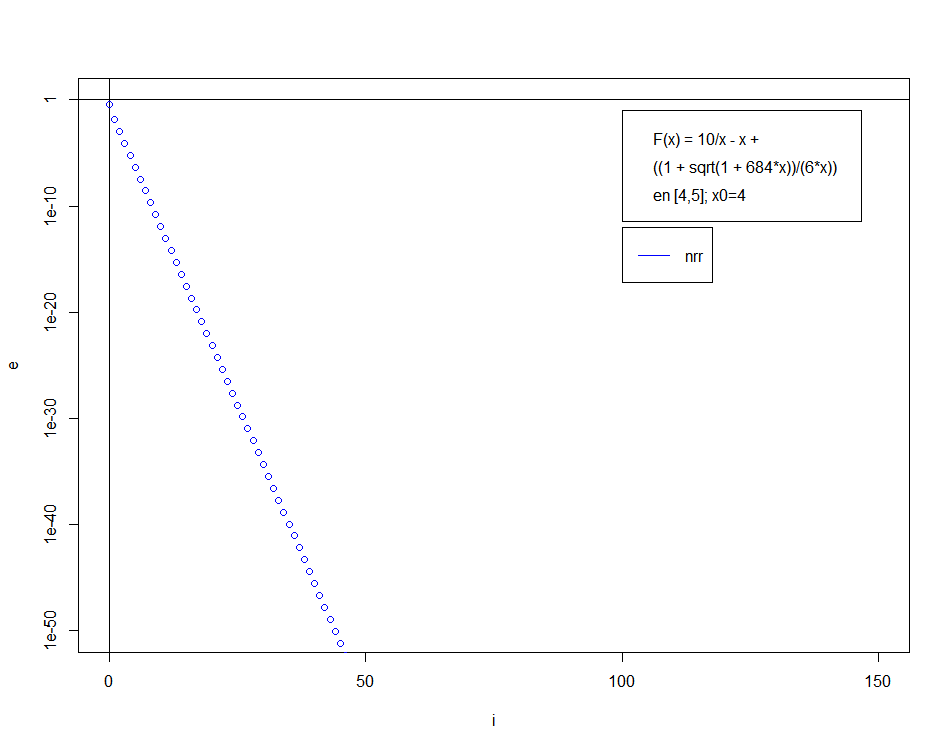
\includegraphics[scale=0.4]{img/nrr_e_vs_i.png}
\vspace{-1em}
\caption{Error vs. Iteraciones del algoritmo de Brent}
\label{fig:nrr_e_vs_i}
\end{figure}

\vspace{-1em}

\subsubsection{Relación entre $\varepsilon_i$ y $\varepsilon_{i+1}$}

A continuación se presenta la gráfica que relaciona $\varepsilon_i$ con $\varepsilon_{i+1}$ para el algoritmo de Brent. \par

% Figura: Relación entre Ei y Ei+1
\vspace{-1em}
\begin{figure}[ht!]
\centering
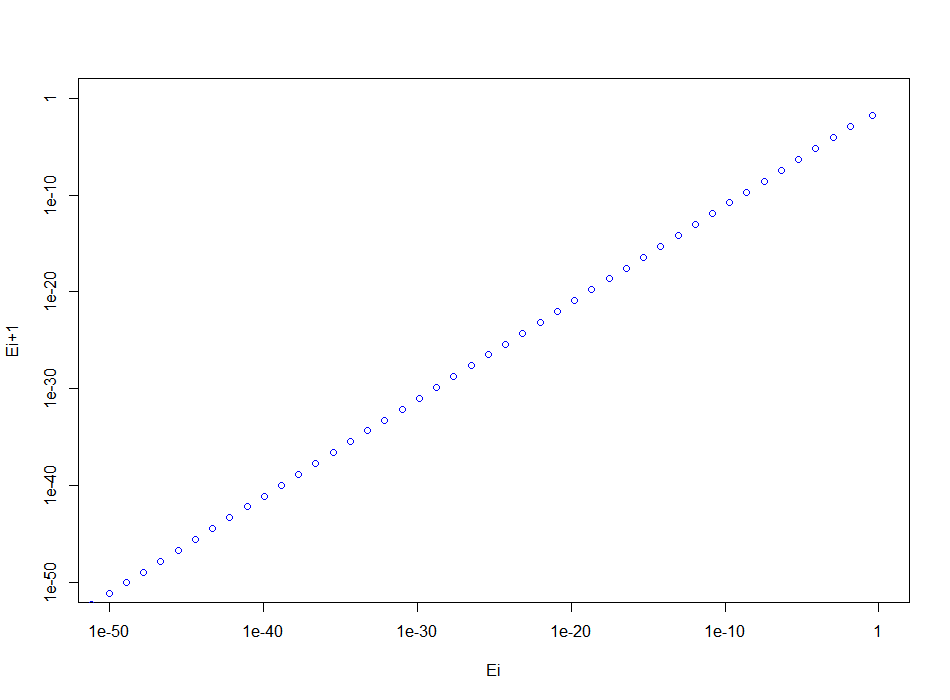
\includegraphics[scale=0.4]{img/nrr_relacion_error.png}
\vspace{-1em}
\caption{Relación entre $\varepsilon_i$ y $\varepsilon_{i+1}$ del método Newton-Raphson Relajado}
\label{fig:nrr_relacion_error}
\end{figure}

\newpage

\subsubsection{Comparación del Método contra el de Bisección}

A continuación se presenta la gráfica que compara la convergencia del algoritmo Newton-Rhapson Relajado, con las del algoritmo de Brent y el método de la bisección. El análisis se realizó a partir de la función $h(x)=\frac{10}{x}-x +\frac{1 + \sqrt{1 + 684 x}}{6x}$ en el intervalo $[4,5]$ con punto inicial $x_0 = 4$. \par

% Figura: NRR vs metodos
\vspace{-1em}
\begin{figure}[ht!]
\centering
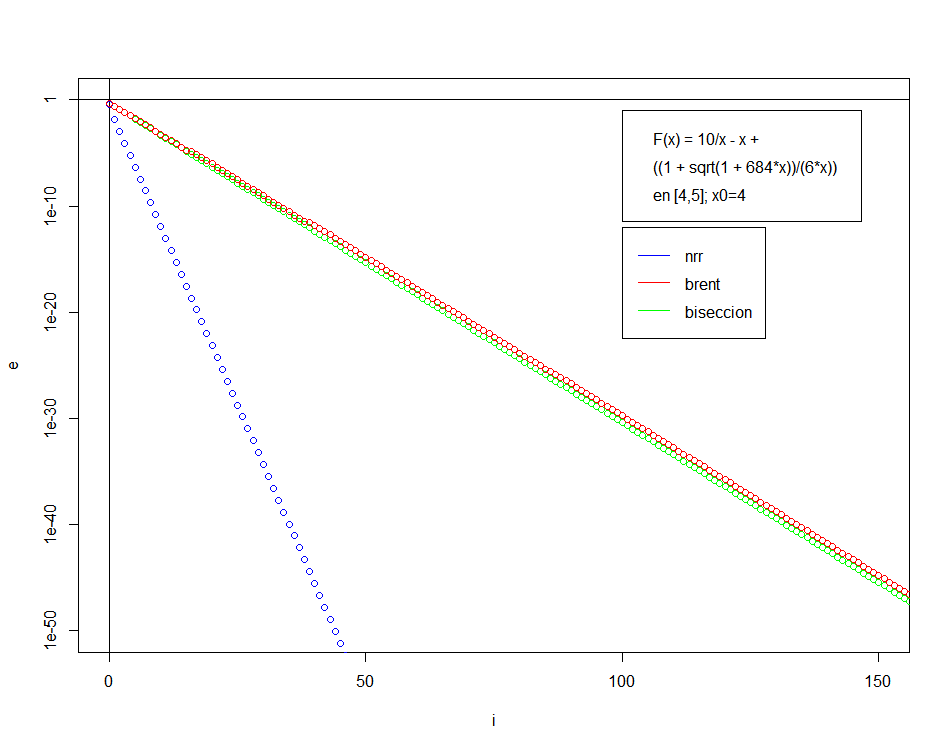
\includegraphics[scale=0.6]{img/nrr_vs_metodos.png}
\vspace{-1em}
\caption{Comparación del algoritmo de Brent contra otros métodos}
\label{fig:nrr_vs_metodos}
\end{figure}

\newpage

%%%%%%%%%%%%%%%%%%%%%%%%%%%%%%%%%%%%%%%%%%%%%%%%%%%%%%%%%%%%%%%%%%%%%%%
% 5.3 Librerías en R
%%%%%%%%%%%%%%%%%%%%%%%%%%%%%%%%%%%%%%%%%%%%%%%%%%%%%%%%%%%%%%%%%%%%%%%

\section{Librerías en R}

La instalación básica de R viene equipada con múltiples funciones para la importación de datos, la realización de transformaciones,la evaluación de polinomios y funciones, las representaciones gráficas, etc. Sin embargo, la enorme potencia de R deriva de su capacidad de incorporar en cualquier momento nuevas funciones capaces de realizar nuevas tareas.
Entre las funciones que explicaremos a continuación se encuentran algunas de las más utilizadas para resolver problemas de raíces e intersecciones, así como también dos paquetes sumamente conocidos como lo son $pracma$ y $rootSolve$.
\par

% Sí, lo dejo ahí para sacar la info de eso. Podríamos hacer un análisis como.
% parametros, salida, funcionamiento
% al final, se pueden quitar los links, y se ponen como referencias

\subsection{Función polyroot}

Polyroot es una función base de R que utiliza el algoritmo de Jenkins-Traub para la aproximación de los ceros de un polinomio.

% https://www.rdocumentation.org/packages/base/versions/3.6.2/topics/polyroot 
\par

\subsubsection{Parámetros}
\begin{itemize}
    \item $z$: vector de coeficientes polinomiales en orden creciente.
\end{itemize}
 
\subsubsection{Salida}

El resultado de la función es un vector complejo de tamaño $n-1$ que contiene las raíces del polinomio, donde $n$ es la posición del elemento de $z$ mas grande distinto de $0$.


\subsection{Función uniroot}
Uniroot es una función base de R que utiliza el método de Brent, el cual combina los métodos de Bisección e Interpolación Cuadrática Inversa para la aproximación de los ceros de una función $f$.
%https://www.rdocumentation.org/packages/stats/versions/3.6.2/topics/uniroot 
\par 

\subsubsection{Parámetros}
 \begin{itemize}
    \item $f$: la función a la que se va a calcular la raíz.
    \item interval: vector que contiene los puntos extremos del intervalo.
    \item ...: argumentos adicionales que pueden ser pasados a $f$.
    \item lower,upper: punto mínimo y punto máximo del intertvalo.
    \item extendInt: cadena de caractéres que especifica si el intervalo debe ser extendido o directamente producir un error cuando $f()$ no tiene signos diferentes en los extemos. Por defecto se inicializa en "no".
    \item check.conv: indicador lógico que establece si la advertencia de convergencia debe ser atrapada como un error y si la no convergencia en el número máximo de iteraciónes debe ser un error en vez de una advertencia.
    \item tol: precisión deseada.
    \item maxiter: número máximo de iteraciones.
    \item trace: número entero, si es positivo se realiza el rastreo de la información.
\end{itemize}

 uniroot(f, interval, …,
        lower = min(interval), upper = max(interval),
        extendInt = c("no", "yes", "downX", "upX"), check.conv = FALSE,
        tol = $.Machinedouble.eps^0.25$, maxiter = 1000, trace = 0)

\subsubsection{Salida}
El resultado de la función es una lista de cuatro componentes:
\begin{enumerate}
    \item root: valor de la raíz calculada.
    \item f.root: valor de la función evaluada en el punto de la raíz.
    \item iter: número de iteraciones realizadas.
    \item estim.prec: precisión estimada para el cálculo de la raíz.
\end{enumerate}

\subsection{Función pracma::brentDekker}

BrentDekker es una función del paquete o librería $pracma$ que implementa una versión del algoritmo de Brent-Dekker, el cual utiliza una combinación del método de la Secante y el método de Bisección junto a la Interporlación Cuadrática para el cálculo de las raíces de una función continua, real y de una sola variable.

%https://www.rdocumentation.org/packages/pracma/versions/1.9.9/topics/brentDekker \par 

\subsubsection{Parámetros}

\begin{itemize}
    \item $f$: función a la que se le calculará la raíz.
    \item a,b: extremo izquierdo y derecho de un intevalo (los valores de la función evaluada en a y b deben ser de signos diferentes).
    \item maxiter: número máximo de iteraciones.
    \item tol: toleracia relativa.
\end{itemize}

brentDekker(f, a, b, maxiter = 100, tol = $.Machinedouble.eps^0.75$) \\
brent(f, a, b, maxiter = 100, tol = $.Machinedouble.eps^0.75$)

\subsubsection{Salida}

El resultado de la función es una lista:
\begin{enumerate}
    \item brent: lista con las raíces de $f$.
\end{enumerate}

\subsection{Función rootSolve::uniroot.all}
rootSolve::Uniroot:all es una función del paquete o librería $rootSolve$ que calcula varias o todas las raíces de una ecuación en un intervalo.

% https://www.rdocumentation.org/packages/rootSolve/versions/1.8.2.1/topics/uniroot.all \par 

\subsubsection{Parámetros}
\begin{itemize}
    \item $f$: función a la que se le calculará la raíz.
    \item interval:  vector que contiene los puntos extremos del intervalo en donde se buscará la raíz.
    \item lower: punto mínimo del intervalo.
    \item upper: punto máximo del intervalo.
    \item tol: precisión deseada.
    \item maxiter: número máximo de iteraciones.
    \item trace: número entero, si es positivo se realiza el rastreo de la información (valores más grandes proporcionan mayor detalle).
    \item n: número de subintervalos en los que se busca la raíz.
    \item ...: argumentos adicionales que puede ser pasados a $f$.
\end{itemize}

uniroot.all(f, interval, lower = min(interval), upper = max(interval), 
            tol = $.Machinedouble.eps^0.2$, maxiter = 1000, 
            trace = 0, n = 100, ...)

\subsubsection{Salida}
El resultado de la función es un vector con las raíces encontradas en el intervalo.

\newpage 

%%%%%%%%%%%%%%%%%%%%%%%%%%%%%%%%%%%%%%%%%%%%%%%%%%%%%%%%%%%%%%%%%%%%%%%
% 5.4 Conclusiones
%%%%%%%%%%%%%%%%%%%%%%%%%%%%%%%%%%%%%%%%%%%%%%%%%%%%%%%%%%%%%%%%%%%%%%%

\section{Conclusiones}

Después de realizar toda la investigación e implementación de los algoritmos utilizando librerias internas y externas para calcular las raíces de un polinomio, así como la ejecución de prácticas y adaptaciones al método de Newton-Raphson Relajado para encontrar intersecciones entre curvas, podemos concluir que existen diferentes metodólogias para resolver problemas de aproximación númerica y que es de suma importancia saber diferenciar cuando debe aplicarse un método en concreto, con el fin de encontrar una solución de manera rápida pero al mismo tiempo precisa y eficiente. \par
Además, quedán definidos, entendidos y practicados distintos métodos directos e iterativos para la resolución de problemas con respecto al cálculo de raíces en polinomios y funciones. \par 

\subsection{Conclusiones del Algoritmo de Brent}

La idea general respecto al método de Brent para la
ubicación de raíces es que siempre que sea posible
utilizar uno de los métodos rápidos abiertos, el algoritmo optará por ese camino, lo que genera una gran ventaja con respecto a otros métodos debido a que significa que es capaz de decidir, por ende, su convergencia será más rápida y en un menor número de iteraciones.
Por otro lado, en el caso de que uno de los métodos abiertos genere un resultado inaceptable, es decir, un estimado de raíces que este fuera del intervalo seleccionado, el algoritmo vuelve al método más conservador de Bisección, lo cual puede ocasionar una perdida importante de significancia y una convergencia más lenta.
 \par

\subsection{Conclusiones de la Intersección entre curvas}

Para hallar la intersección entre curvas es necesario la implementación de varios algoritmos. para la resolución de este problema pudimos implementar un metodo iterativo como lo es el Newton-Rhapson Relajado, el cual nos permitio de manera sencilla pero muy completa encontrar una aproximación de la raíz con un error menor a \(2^{-16}\) y entender como es que se halla el punto de intersección.\par

\subsection{Conclusiones de las Librerías utilizadas}

Las librerías como $pracma$ o $solveRoot$ disponibles para el trabajo con raíces en el lenguaje R son de gran utilidad en el momento de implementar soluciones de problemas relativamente sencillos, puesto que facilitan la utilización de métodos más complejos que ya vienen impletados dentro de las funciones que estos paquetes proporcionan, siendo sumamente sencillas de aplicar, sin embargo, las cifras significativas y la toleracia con las que trabajan este tipo de funciones por lo general ofrecen una precisión bastante baja, lo que para este curso es inaceptable y nos obliga a utilizar otras implementaciones mejoradas con el fin de llegar a una solución más exacta. \par

\newpage

%%%%%%%%%%%%%%%%%%%%%%%%%%%%%%%%%%%%%%%%%%%%%%%%%%%%%%%%%%%%%%%%%%%%%%%
% 6 Referencias
%%%%%%%%%%%%%%%%%%%%%%%%%%%%%%%%%%%%%%%%%%%%%%%%%%%%%%%%%%%%%%%%%%%%%%%

\bibliographystyle{IEEEtranN}
\bibliography{References}

\end{document}

%%%%%%%%%%%%%%%%%%%%%%%%%%%%%%%%%%%%%%%%%%%%%%%%%%%%%%%%%%%%%%%%%%%%%
% Ejemplos
%%%%%%%%%%%%%%%%%%%%%%%%%%%%%%%%%%%%%%%%%%%%%%%%%%%%%%%%%%%%%%%%%%%%%

%%%%%%%%%%%%%%%%%%%%%%% Insertar Imágenes %%%%%%%%%%%%%%%%%%%%%%%%%%
%\begin{figure}[h!]
%\centering
%\includegraphics[scale=1.7]{img/ruta.jpg}
%\caption{Nombre de la figura}
%\label{fig:etiqueta}
%\end{figure}
